\subsection{Resources} \label{Resources section}
Most of our required resources are open-sources:
\begin{itemize}
    \item Python 3.6+:\\ \url{https://www.python.org/downloads/}
    \item Jupyter Notebook:\\ \url{https://jupyter.org/}
    \item Qiskit:\\
          \url{https://qiskit.org/}
    \item IBM Quantum:\\ \url{https://quantum-computing.ibm.com/}
    \item Qiskit circuit library:\\ \url{https://qiskit.org/documentation/apidoc/circuit_library.html}
\end{itemize}

To prepare the quantum emulator on a local machine, we first install Python and Anaconda for programming language support and Jupyter Notebook as a code editing tool.
Then we follow the official instruction from Qiskit \cite{Qiskit} to install the necessary packages.
The quantum emulator from Qiskit is capable of simulating up to 32 qubits.
We can start working with Qiskit in a Jupyter Notebook file.

The other option is to use the provided Python notebook environment provided by IBM Quantum with Qiskit pre-installed.
While this is a convenient choice for online presentation or remote working because of instant access, this server has shortcomings.
The maximum amount of RAM for open access is only 8 Gigabytes, and the processing power is limited.
The actual quantum hardware from IBM is limited to 5 qubits for open access.

Qiskit offers various pre-defined ansatz designs, namely \textit{EfficientSU2, PauliTwoDesign, RealAmplitudes, NLocal}, \textit{TwoLocal}, etc.
The Qiskit circuit library also allows custom parameterized circuits to be used as ansatzes.
Each of the circuit templates is used for different purposes, such as quantum chemistry, quantum neural network, quantum eigensolver, etc.
They also have their advantages or disadvantages.
For example, it is common to use the \textit{RealAmplitudes} ansatz to implement a multi-layer perceptron neural network.

\subsubsection{Creating Ansatzes} \label{Sec: Creating Ansatzes}
We have chosen the \textit{Real Amplitudes} ansatz from Qiskit circuit library.
An example of circuits generated by Qiskit is visualised in Figure \ref{Fig: Ansatz samples}.
We can generate different ansatz by altering the repetition number and qubit number.
The circuit depth is the largest number of gate operations across all qubit registers in a circuit.
Furthermore, as the circuit high-level definition is translated into the gate set available on a given quantum machine, the circuit depth may significantly increase.
Obviously, as the ansatz repetition grows, the circuit depth also grows.
Figure \ref{Fig: Ansatz samples} further shows that the higher number of qubits leads to a deeper circuit for a linear entangled ansatz.

\begin{figure}
    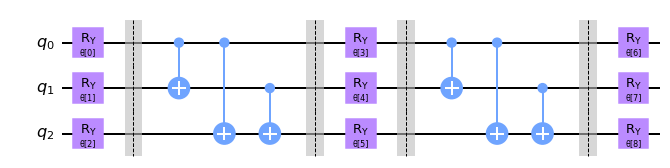
\includegraphics[width=\linewidth]{Artefact/Appendices/ansatz3-2.png}
    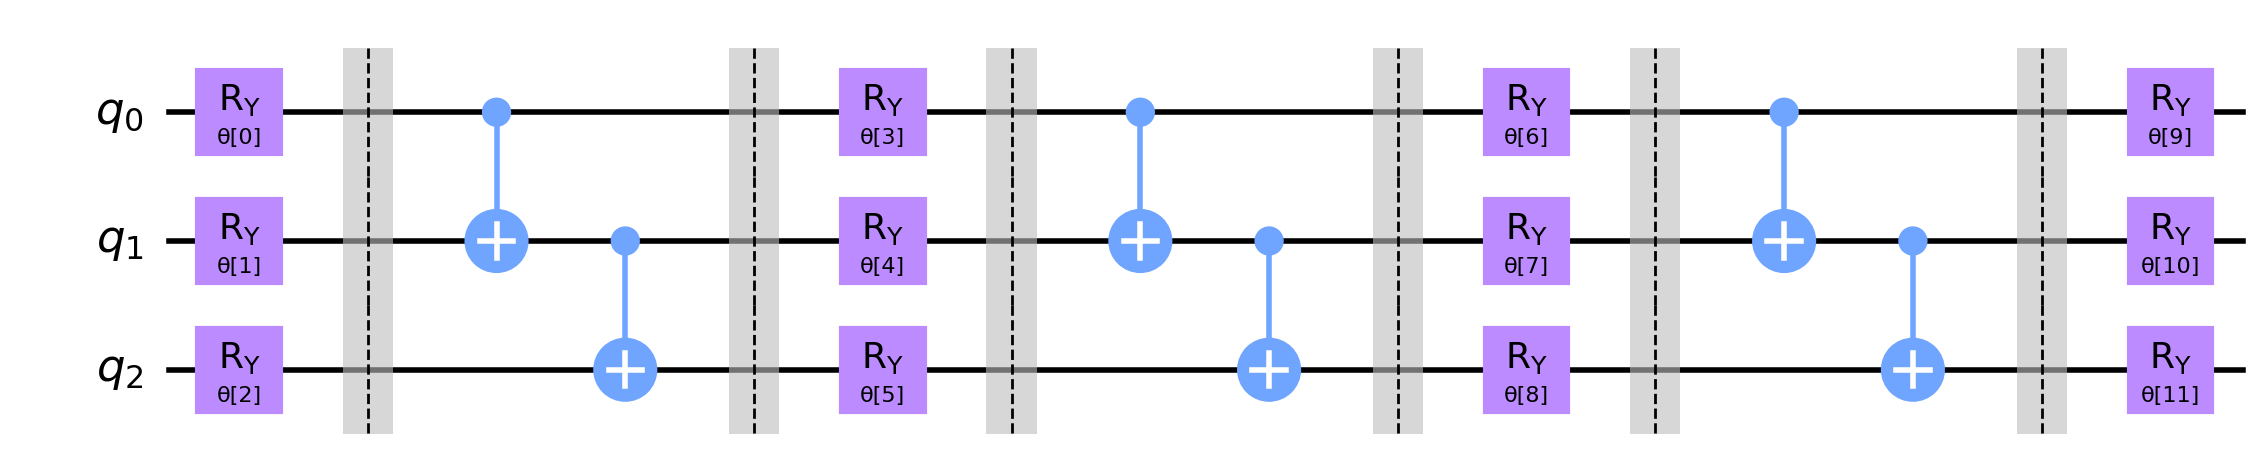
\includegraphics[width=\linewidth]{Artefact/Appendices/ansatz3-3.png}
    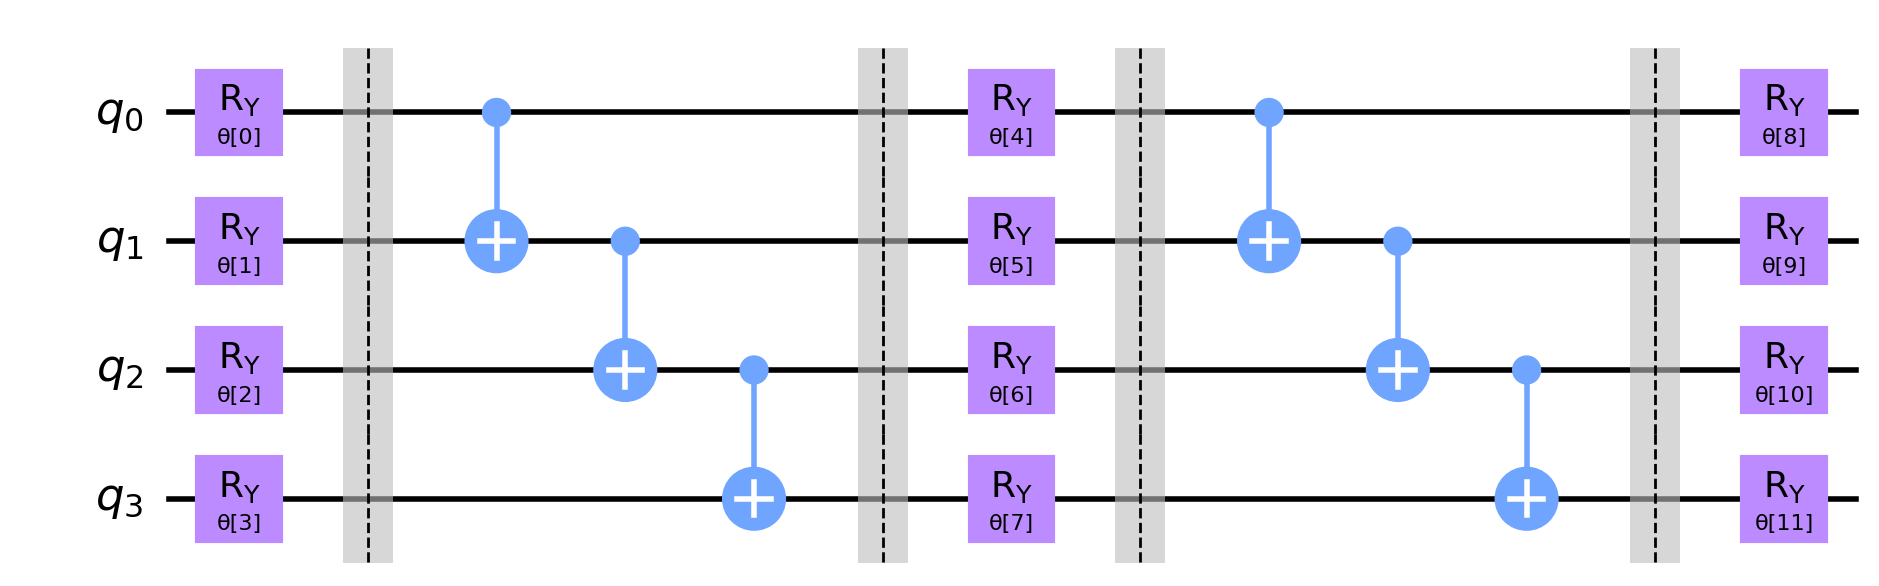
\includegraphics[width=\linewidth]{Artefact/Appendices/ansatz4-2.png}
    \caption{
        Samples of parameterised circuits generated by the Qiskit framework.
        The ansatz is a sequence of rotation layers and entanglement layers.
        All three: Real Amplitudes ansatz generated by Qiskit.
        Above: an ansatz of three qubits and two repetition layers.
        Middle: an ansatz of three qubits and three repetition layers.
        Below: an ansatz of four qubits and two repetition layers.
    }
    \label{Fig: Ansatz samples}
\end{figure}

For the case of identity block method, we will be using a customised ansatz, since reversing an ansatz would cancel the effect of the entanglement layer.
The customised ansatz are specialised to create identity blocks without losing the entanglement layers, section \ref{Sec: Method3} gives further discussion of this ansatz.

\subsubsection{The Quantum Provider}
For this experiment, we are using the quantum emulator provided by Qiskit.
The QASM simulator is used to mimic an IBMQ device.
Additionally, the QASM simulator, by default, has no noise, so we configure the emulator to receive  noise profile from the backend \emph{ibm\_perth}.
Note that the emulators do not reflect quantum devices precisely as the actual devices, for example, execution time, decoherence time and queue time.
However, considering the allowed time span for these experiments, we will use the QASM simulator for the experiment and leave the actual quantum devices for future works.